\documentclass[11pt]{article}

\usepackage[a4paper,margin=1in]{geometry}
\usepackage{amsmath,amssymb,mathtools}
\usepackage{array}
\usepackage{booktabs}
\usepackage{enumitem}
\usepackage{tikz}
\usepackage{physics}
\usetikzlibrary{arrows.meta,positioning}

\setlength{\parindent}{0pt}
\setlength{\parskip}{0.75em}

\newcommand{\answersection}{%
    \subsection*{Answer}
    % Write your answer here.
}

\title{CO250 Assignment 1}
\date{September 14--21}

\begin{document}

\maketitle

\section*{Problem 1}

Waterloo's infamous Maple Syrup Madness produces maple syrup for the entire southern part
of Ontario. The following table shows the demand $d_i$ (in tons) for each month
$i\in\{1,\ldots,12\}$.

\begin{center}
\begin{tabular}{c|*{12}{c}}
\toprule
Month & 1 & 2 & 3 & 4 & 5 & 6 & 7 & 8 & 9 & 10 & 11 & 12 \\
\midrule
$d_i$ & 10 & 12 & 14 & 20 & 15 & 18 & 19 & 20 & 30 & 28 & 31 & 22 \\
\bottomrule
\end{tabular}
\end{center}

The company needs to decide how much maple syrup to produce in each month so that the
demand can be met. As usual we make the following assumption: maple syrup produced in
month $i$ can be consumed in month $i$ (and later, of course).

\subsection*{(a)}

Assume that producing a ton of maple syrup in month $i$ costs $p_i$, and that the company
can store up to 15 tons of its product in its storage facility for an unlimited amount of
time. Assume that the storage facility contains 7 tons of maple syrup at the beginning of
month 1.

The company wants to determine how much to produce in each month in order to minimize
the total production cost. Write an LP for this task.

\answersection

Let $s_i$ be the amount of maple syrup (in tons) in storage at the end of month $i$.\\
Let $x_i$ be the amount of maple syrup produced in month $i$.

\begin{align*}
    \text{Objective:}\qquad
        & \min \sum_{i=1}^{12} p_i x_i \\
    \text{subject to:}\qquad
        & s_i = s_{i-1} + x_i - d_i && \forall i\in [12] \\
        & 0 \leq s_i \leq 15 && \forall i\in [12]\\
        & s_0 = 7 \\
        & x_i \geq 0 && \forall i\in [12].
\end{align*}

\subsection*{(b)}

Now assume that the company wants to even out production over the year in order to
keep its demand for staff constant. We model this by assuming that the company incurs
a cost of 50 for each ton of difference between the production quantities in any two
consecutive months. As an example, assume that the company decides to produce $x_i$
tons of maple syrup in month $i\in\{1,\ldots,12\}$.

\begin{center}
\begin{tabular}{c|*{12}{c}}
\toprule
$i$ & 1 & 2 & 3 & 4 & 5 & 6 & 7 & 8 & 9 & 10 & 11 & 12 \\
\midrule
$x_i$ & 4 & 19 & 21 & 16 & 32 & 32 & 20 & 10 & 12 & 5 & 6 & 8 \\
\bottomrule
\end{tabular}
\end{center}

The cost incurred by the company for the production plan given in the above table is
\[
\begin{aligned}
\bigl(
&(19-4)+(21-19)+(21-16)+(32-16)+(32-32)+(32-20)\\
&+(20-10)+(12-10)+(12-5)+(6-5)+(8-6)
\bigr)\cdot 50.
\end{aligned}
\]

As in (a), assume that the storage facility contains 7 tons of maple syrup at the beginning
of month 1, and that you can store up to 15 tons of maple syrup at any time.

The company wants to find a production schedule that minimizes the total cost incurred
by production changes. Formulate the problem as an LP.

\answersection
Introduce auxiliary variables $y_i$ that, through constraints, will represent $y_i = \abs{x_i - x_{i+1}}$.

\begin{align*}
    \text{Objective:}\qquad
        & \min \sum_{i=1}^{11} 50y_i \\
    \text{subject to:}\qquad
        & y_i \geq x_i - x_{i+1} && \forall i\in [11] \\
        & y_i \geq x_{i+1} - x_i && \forall i\in [11] \\
        & s_i = s_{i-1} + x_i - d_i && \forall i\in [12] \\
        & 0 \leq s_i \leq 15 && \forall i\in [12]\\
        & s_0 = 7 \\
        & x_i \geq 0 && \forall i\in [12].
\end{align*}

\newpage
\section*{Problem 2}

Consider the following word game. You are assigned a number of tiles, each containing letters
from the alphabet
\[
\Sigma=\{a,b,c,\ldots,z\}.
\]
Suppose that your input contains $N_\alpha\in\mathbb{N}$ tiles with the letter $\alpha$
for each $\alpha\in\Sigma$. From the letters you are to construct any of the words
$w_1,\ldots,w_n$. This list might for example consist of all the words in a dictionary.

You must construct any word at most once, and use any tile at most once. You receive
$v_j\ge 0$ points for constructing word $w_j$, and an additional bonus $b_{ij}\ge 0$
for making both words $w_i$ and $w_j$.

\subsection*{(a)}

Formulate an integer program to determine your optimal choice of words (one that maximizes
the total number of points + bonus).

\answersection

\subsection*{(b)}

How does your formulation change when you are allowed to select 100 tiles with no
restriction on your choice of letters?

\answersection


\newpage
\section*{Problem 3}

\begin{figure}[h]
\centering
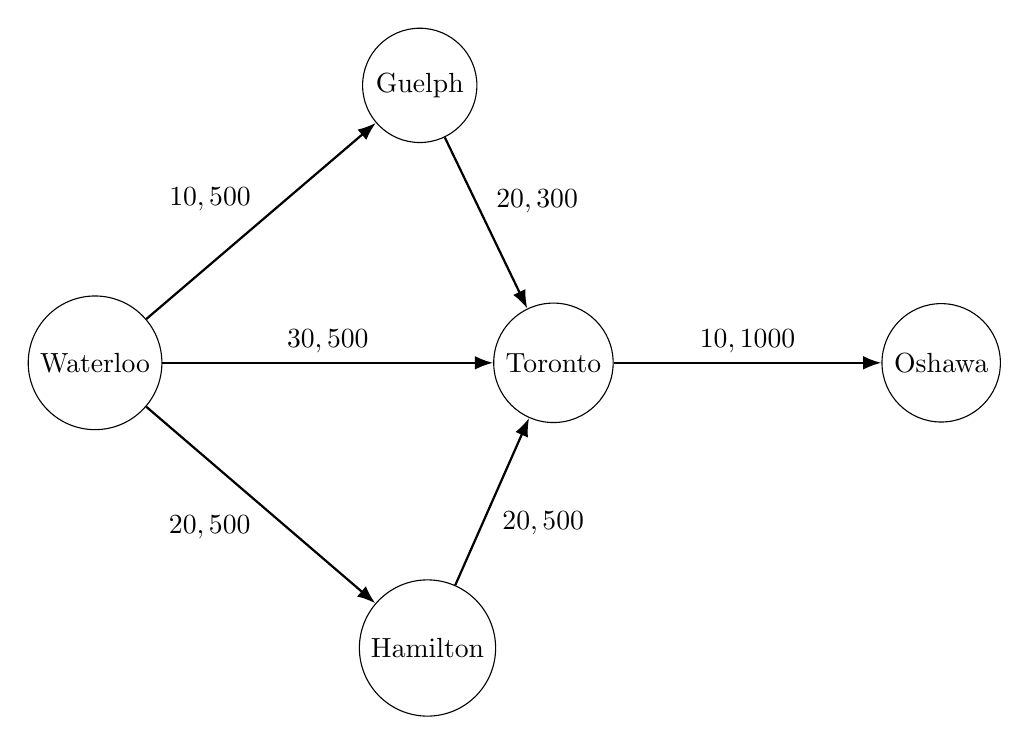
\begin{tikzpicture}[
    >=Latex,
    node distance=2.4cm and 3.0cm,
    city/.style={circle,draw,minimum size=1.1cm,align=center},
    every edge/.style={draw,->,thick}
]
\node[city] (W) {Waterloo};
\node[city, above right=of W] (G) {Guelph};
\node[city, below right=of W] (H) {Hamilton};
\node[city, right=4.2cm of W] (T) {Toronto};
\node[city, right=3.4cm of T] (O) {Oshawa};

\draw[->,thick] (W) -- node[above left] {$10,500$} (G);
\draw[->,thick] (W) -- node[below left] {$20,500$} (H);
\draw[->,thick] (W) -- node[above] {$30,500$} (T);
\draw[->,thick] (G) -- node[above right] {$20,300$} (T);
\draw[->,thick] (H) -- node[below right] {$20,500$} (T);
\draw[->,thick] (T) -- node[above] {$10,1000$} (O);
\end{tikzpicture}
\caption{Maple Syrup Madness Pipe Network for Problem 3. The numbers $10,500$ on the arc
connecting Waterloo to Guelph signal that it costs 10 cents to send a litre from Waterloo
to Guelph, and that it is possible to send up to 500 litres.}
\end{figure}

Maple Syrup Madness has a plant in each of the cities of Waterloo, Guelph, Hamilton,
Toronto, and Oshawa. Maple Syrup Madness marketing team has proposed that selling maple
syrup for 100 cents in Oshawa may be a good idea for the company brand. To attend this
demand, the company will employ its remarkable pipe infrastructure connecting its plants
(see Figure 1). Namely:

\begin{itemize}
    \item the Waterloo plant can send maple syrup to Guelph, Hamilton, and Toronto, at the
    cost of 10, 20, and 30 cents per litre, respectively;
    \item the Guelph plant can send maple syrup to Toronto at the cost of 20 cents per litre;
    \item the Hamilton plant can send maple syrup to Toronto at the cost of 20 cents per litre;
    \item the Toronto plant can send maple syrup to Oshawa at the cost of 10 cents per litre.
\end{itemize}

The Waterloo plant has a total of 1000 litres of maple syrup that can be used in this publicity
stunt. But given the short window between when these litres are produced and when they
must be sold in Oshawa, the pipe capacities impose restrictions on how many litres can be
sent in each pipe. Each of the pipes listed above has a maximum capacity of 500 litres;
except the pipe between Guelph and Toronto, that can only be used to send 300 litres, and
the recently upgraded pipe between Toronto and Oshawa, which can be used to send
1000 litres.

The company would like to know the maximum profit it can achieve from selling Waterloo's
maple syrup in Oshawa for 100 cents. Formulate an LP to solve that task.

\answersection


\newpage
\section*{Problem 4: Review of linear algebra}

\subsection*{(a) Bases and subspaces}

Show that the vectors
\[
A_1 :=
\begin{pmatrix}
1\\
0\\
1
\end{pmatrix},
\qquad
A_2 :=
\begin{pmatrix}
1\\
2\\
1
\end{pmatrix},
\qquad
A_3 :=
\begin{pmatrix}
-1\\
-1\\
1
\end{pmatrix}
\]
form a basis for $\mathbb{R}^3$.

\answersection

\subsection*{(b)}

Express each of the following vectors as linear combinations of $A_1$, $A_2$, and $A_3$:
\[
A_4 :=
\begin{pmatrix}
1\\
0\\
0
\end{pmatrix},
\qquad
A_5 :=
\begin{pmatrix}
0\\
1\\
0
\end{pmatrix},
\qquad
A_6 :=
\begin{pmatrix}
0\\
0\\
1
\end{pmatrix}.
\]

\answersection

\subsection*{(c)}

Let $m$ and $k$ be a pair of positive integers.

Let $\{A_1,A_2,\ldots,A_k\}\subset\mathbb{R}^m$ be a linearly independent subset of vectors.
Suppose $A_{k+1}\in\mathbb{R}^m$ is not in the subspace spanned by the vectors
$\{A_1,A_2,\ldots,A_k\}$. Prove that the set
\[
\{A_1,A_2,\ldots,A_k,A_{k+1}\}
\]
is linearly independent.

\answersection

\subsection*{(d)}

Prove that every linearly independent subset of vectors in $\mathbb{R}^m$ is part of a basis.
So, given a linearly independent subset of vectors (say $k$ of them) in $\mathbb{R}^m$, we
can always find $m-k$ vectors to extend the initial subset to a basis for $\mathbb{R}^m$.

\answersection

\end{document}
